\begin{figure}[!ht]
	\centering
	\begin{subfigure}{\textwidth}
		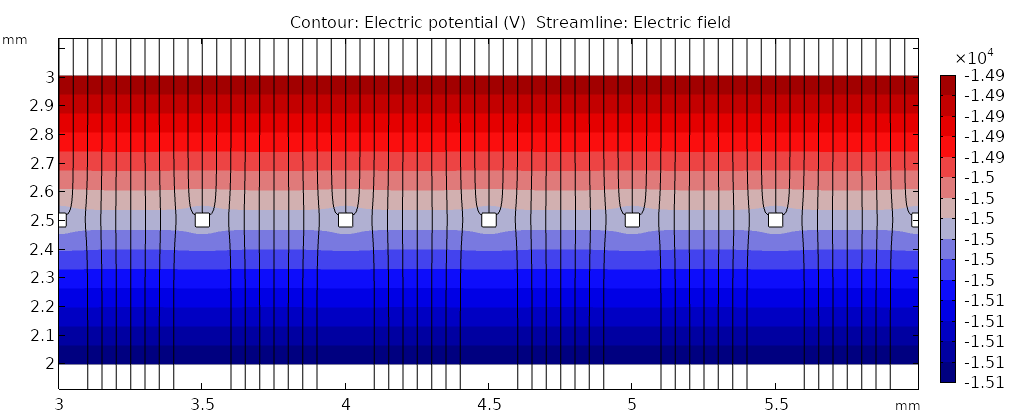
\includegraphics[width=\textwidth]{03_Prototype/figures/fig027_Grid1.png}
		\caption[]{Configuration 1: The field is constant (up: \(3\,\mathrm{kV/cm}\); down: \(3\,\mathrm{kV/cm}\)). The mesh transmission is close to the optical transparency.}
		\label{chap3:Grid1}
	\end{subfigure}

	\begin{subfigure}{\textwidth}
		\centering
		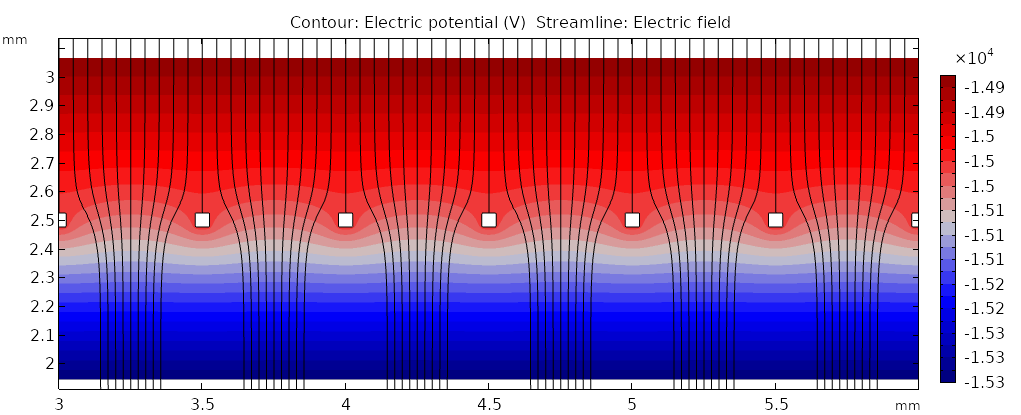
\includegraphics[width=\textwidth]{03_Prototype/figures/fig027_Grid2.png}
		\caption[]{Configuration 1: The field is higher below the grid (up: \(3\,\mathrm{kV/cm}\); down: \(6\,\mathrm{kV/cm}\)). The mesh transmission is higher than the optical transparency.}
		\label{chap3:Grid2}
	\end{subfigure}
	\caption[Electrical simulations of a \(50/450\,\mathrm{\mu m}\) grid]{Electrical simulations of a \(50/450\,\mathrm{\mu m}\) grid. Two different field configurations were simulated. Both shows that the electrical field becomes uniform few mm away from grid. However the particle transmission differs due different ratios of the electric fields imposed in the two regions.}
	\label{chap3:Grid}
\end{figure}
